%\chapter{La caméra NIKA2 au télescope de 30 mètres de l'IRAM}

\begin{figure}[ht!] 
\begin{center}
\includegraphics[clip,trim={0, 1cm, 0, 2cm},width=0.5\textwidth]{Figures/NIKA2/mm_universe_LPSC_v2_notexte_clement_petit2.pdf}
\caption[Illustration du télescope de 30 mètres de
  l'IRAM]{Illustration du télescope de 30 mètres de l'IRAM. Crédit :
  Clément C. Favre.} 
 \label{fig:affiche}
\end{center}
\end{figure}


L'expérience NIKA2 est installée au télescope de 30-m de l'IRAM, sis à
2800 mètres d'altitude à Pico Veleta en Espagne, et ce, depuis
octobre 2015. Après une phase de \emph{commissioning} marquée par
plusieurs interventions sur l'instrument, les observations
scientifiques ont commencées en octobre 2017. NIKA2 est dès lors l'un
des instruments à demeure du télescope de 30-m de l'IRAM et restera
ouvert à la communauté scientifiques jusqu'à 2030 environ.

Les choix technologiques de NIKA2 s'appuient largement sur
l'expérience acquise avec NIKA, l'instrument précurseur, environ un
ordre de grandeur plus petit que NIKA2 dans sa version
finale~\citep{Monfardini2014JLTP}. NIKA a été extensivement testé
au laboratoire puis au télescope de 30-m~\citep{Catalano2014}. Ces
performances ont motivées qu'il soit ouvert à la communauté pour une
saison d'observations scientifiques à l'hiver 2014.

Ce chapitre s'ouvre sur une brève description l'instrument NIKA2
(Sect.~\ref{se:instrument}), puis continue en donnant quelques bases
des techniques d'observation utilisées au télescope de 30-m
(Sect.~\ref{se:observations}). La Sect.~\ref{se:commissioning} résume
le déroulement de la phase de \emph{commissioning}, aborde quelques
aspects relevant de l'organisation du travail que j'ai mise en place,
et se conclut par la sélection du jeu de données de référence pour la
caractérisation des performances.



\section{L'instrument}
\label{se:instrument}

La conception de NIKA2 répond à l'exigence de cartographier dans deux
bandes de frequences, un champ de vue de plusieurs minutes d'arc, sans
dégrader la résolution angulaire permise par le télescope de 30-m,
avec une sensibilité suffisante pour la détection de sources compactes
en dessous du milli-Jansky et l'étude de sources diffuses faibles.

Le signal millimétrique étant fortement absorbé par l'atmosphère, les
bandes de fréquences d'observation ont été choisies centrées
autour de 150 et 260 GHz, dans les fenêtres de transmission maximale
du signal. A ces fréquences, la couverture d'un grand champ de vue
avec une résolution angulaire proche de la limite de diffraction du
télescope nécessite le déploiement de plusieurs milliers de détecteurs
au plan focal.

NIKA2 est équipée d'environ 2900 détecteurs supraconducteurs à inductance
cinétique, les \emph{kinetic inductance detectors} (KID) distribués
dans trois matrices de détecteurs. NIKA2 au télescope de 30-m permet
une cartographie à une résolution angulaire de l'ordre de la dizaine
de secondes d'arc dans un champ de vue de 6,5 minutes d'arc, dans deux
bandes de fréquence centrées à 150 et 260 GHz et avec une sensibilité
au niveau des meilleures expériences millimétriques actuelles.

Le dispositif instrumental est décrit de manière détaillée dans
\citet{Adam2018}. Ici, je présente brièvement les principaux
sous-ensembles instrumentaux en me concentrant sur ceux qui font la
spécificité de NIKA2 ou qui imposent des contraintes sur la
calibration ou l'analyse des données de NIKA2.


\subsection{Les \emph{kinetic inductance detectors}}
\label{se:kid}

Fort du succès de NIKA, NIKA2 utilise les KID, qui offrent une
alternative intéressante aux bolomètres, équipant la plupart des
expériences CMB actuelles, pour la fabrication de grandes matrices de
détecteurs~\citep{Day2003, Doyle2008_LEKID}. 

Le principe physique des KID est fondé sur une propriété des matériaux
supraconducteurs en couche mince. Dans un supraconducteur, les
électrons s'associent en paires de Cooper, assurant le transport de
charges. La dynamique des paires de Cooper dans un champ
electromagnétique variable confert au matériau une impédance non-nulle
via une inductance cinétique. Les photons incidents dont
l'énergie dépasse le sueuil de transition du supraconducteur (dépendant
du matériau) peuvent briser des paires de Cooper, modifiant la densité
de quasi-particules et \emph{in fine} de l'impédance de surface du
matériau. Dans un circuit RLC gravé dans un tel matériau
supraconducteur, ce changement d'impédance sous l'effet de variations
de l'inductance cinétique se traduit en un changement
de la fréquence de résonance du circuit. Un tel résonateur
supraconducteur forme un KID. 

Les KID qui équipent NIKA et NIKA2 sont
de type \emph{Lumped Element Kinetic Inductance
  Detector}~\citep{Doyle2008_LEKID,Roesch2012_LEKID}. Dans
ce type de KID, les photons incidents sont absorbés dans un méandre
qui forme la partie inductive du circuit RLC, de sorte de maximiser
l'impact des variations d'inductance cinétique du matériau.   
Une fois le KID connecté à une ligne de transmission, les variations
de sa fréquence de résonance sous l'effet de l'absorption de photons
sont mesurées par comparaison entre un signal d'excitation à
une fréquence proche de la fréquence de résonance du KID dans
l'obscurité et le signal transmis. 
De plus, un KID peut être conçu
pour n'occuper qu'une fine bande en fréquence sur la ligne de
transmission et pour avoir une fréquence de résonance bien déterminée,
de sorte qu'il est possible de connecter un grand nombre de KID sur
une même ligne de transmission : les KID sont donc multiplexés dans le
domaine fréquenciel. Couplés avec une électronique de lecture
dédiée~\citep{Bourrion2016}, les signaux de plusieurs centaines de KID
peuvent être lus simultanément. 
%En sus
%d'être hautement multiplexables, les KID présentent plusieurs
%avantages, tels la simplicité de fabrication au sein de grandes
%matrices de détecteurs, les courtes constantes de temps, etc., comme
%discuté dans \reference{monfardini2010}.
La technologie des matrices de KID utilisée par NIKA2 a été validée
avec l'instrument
NIKA~\citep{Monfardini2010_NIKA, Monfardini2011_NIKA, Roesch2012_LEKID, Calvo2013}.



\subsection{Le cryostat}
   
\begin{figure}[ht!] 
\begin{center}
\includegraphics[clip,width=0.7\textwidth]{Figures/NIKA2/cryostat_fr.pdf}
\caption[Coupe transversale du cryostat]{Coupe transversale du
  cryostat et simulation de rayons optiques.} 
 \label{fig:cryostat}
\end{center}
\end{figure}

Pour une sensibilité optimale, les KID doivent être refroidis à une
température bien en-deça de la température critique du matériau
supraconducteur qui les compose. Dans le cas des détecteurs de NIKA2,
formés par un fin film d'aluminium, cette température optimale de
fonctionnement se situe autour de 150~mK. De plus, pour réduire le
rayonnement parasite dans le détecteur, une partie de l'optique est
également maintenue à 150~mK. Ce refroidissement est assuré par
un cryostat à dilution $^3$He/$^4$He, fonctionnant en cycle
fermé, spécialement conçu pour NIKA2 à l'Institut Néel. La partie
centrale du cryostat à 150~mK, pesant près de 100~kg, est entourée de
deux étages cryogéniques maintenus à 4.2~K et à 70~K, respectivement, au
moyen de deux \emph{pulse tubes}. A chaque étage, sont ajoutés des
systèmes d'écrantage pour se prémunir du champ magnétique terrestre et
de ses variations dans le référentiel de l'instrument lors du
mouvement du télescope pendant les observations. Enfin, les surfaces
internes sont recouvertes d'un matériau limitant les réflexions de
lumières parasites au sein du cryostat. L'ensemble du cryostat, dont
une coupe transversale est montrée à la figure~\ref{fig:cryostat}, forme
un imposant système mesurant 2,3 mètres de long et pesant plus d'une
tonne, entièrement dessiné à l'Institut Néel. La température des
détecteurs présente une stabilité remarquable, avec des variations de
l'ordre de la fraction de mK pour la durée typique d'une observation
(quelques dizaines de minutes)~\citep{Adam2018}.

\subsection{L'optique}
\label{se:optics}

La lumière collectée par le miroir primaire du télecope de 30-m
illumine les détecteurs de NIKA2 via un ensemble optique dédié. Après
le miroir secondaire (M2), quatre miroirs situés dans la cabine du
télescope dirrige la lumière vers l'entrée du cryostat. L'optique
froide, placée à l'intérieure du cryostat, est illustrée à la
figure~\ref{fig:cryostat}. Elle comprend six lentilles et deux miroirs
(M7 et M8), maintenus à 30~K, placés à l'avant du cryostat et qui
dirrigent la lumière vers les parties centrales. Une série de filtres
passe-bande sont placés à chaque étages cryogéniques pour supprimer la
lumière parasite. 
Dans la partie à 150~mK, une lame dichroïque orientée à 45
degrés par rapport à l'axe optique assure la séparation du faisceau
lumineux en deux bandes : la composante à 150~GHz est réfléchie
tandis que celle à 260~GHz est transmise. Cet élément optique, d'un
diamètre de 30~cm et refroidi à 150~mK, a été spécialement conçu à
Cardiff pour résister aux déformations dues aux très basses
températures. Il utilise une nouvelle technologie, dite
\emph{air-gap}, et une monture renforcée~\citep{Perotto2019}. Pour chaque faisceau, est
ajouté un diaphragme d'ouverture conçu pour limiter légèrement la
pupille d'entrée du télescope de 30-m à un diamètre de 27,5 mètres.   
Le faisceau à 260~GHz traverse ensuite un polariseur
orienté à 45 degrés par rapport à l'axe optique afin de séparer la lumière en
deux faisceaux polarisés linéairement : la composante horizontale dans
le référentiel lié au cryostat est transmise tandis que la composante
verticale est réfléchie par le polariseur.
Finalement, un dernier filtre qui détermine la bande passante est
placé devant chaque matrice de détecteurs.

\subsection{Les matrices de détecteurs et l'électronique}
\label{se:matrices}

NIKA2 est équipé de trois matrices de KID. L'une, placée au plan focal du
faisceau à 150\,GHz, est appélée \emph{Array 2} (A2), en référence à la
longueur d'onde correspondante, 2~mm. Les deux autres collectent les
deux composante de lumière polarisée linéairement dans la bande
passante à 260\,GHz : la composante horizontale (transmise par le
polarimètre) éclaire \emph{Array 1} (A1) et la composante verticale
(refléchie par le polarimètre) \emph{Array 3} (A3). Le positionnement
des matrices est indiqué à la figure~\ref{fig:cryostat}. 

Le nombre de pixels (détecteurs) qui composent chacune des matrices
dépend de leur taille, qui elle-même résulte d'une double contrainte :
la pixelisation doit être suffisament fine pour atteindre la limite de
diffraction du télescope tandis que l'aire collectrice de lumière de
chaque pixel doit être large pour assurer une bonne sensibilité. Aux
longueurs d'onde centrées à 2~mm, les pixels mesurent 2,8~mm de coté,
correspondant à l'optimum permis. A 1~mm, les pixels font 2~mm de coté
assurant un échantillonage du plan focal proche de l'optimalité
(environ 1,1 $\lambda/D$, pour $D = 27,5~\rm{m}$, le diamètre de la
pupille d'entrée). Pour couvrir le champ de vue de 6,5 arcmin, la
matrice à 2~mm (A2) se compose de 616 détecteurs et chacune des deux
matrices à 1~mm (A1\&A3) de 1140 détecteurs arrangés en un disque
(Fig.~\ref{fig:ma_fig}).

%{\color{vert}\lipsum[1-2]}

\begin{figure}[!ht]
  \begin{minipage}[c]{0.50\linewidth}
    \centering
    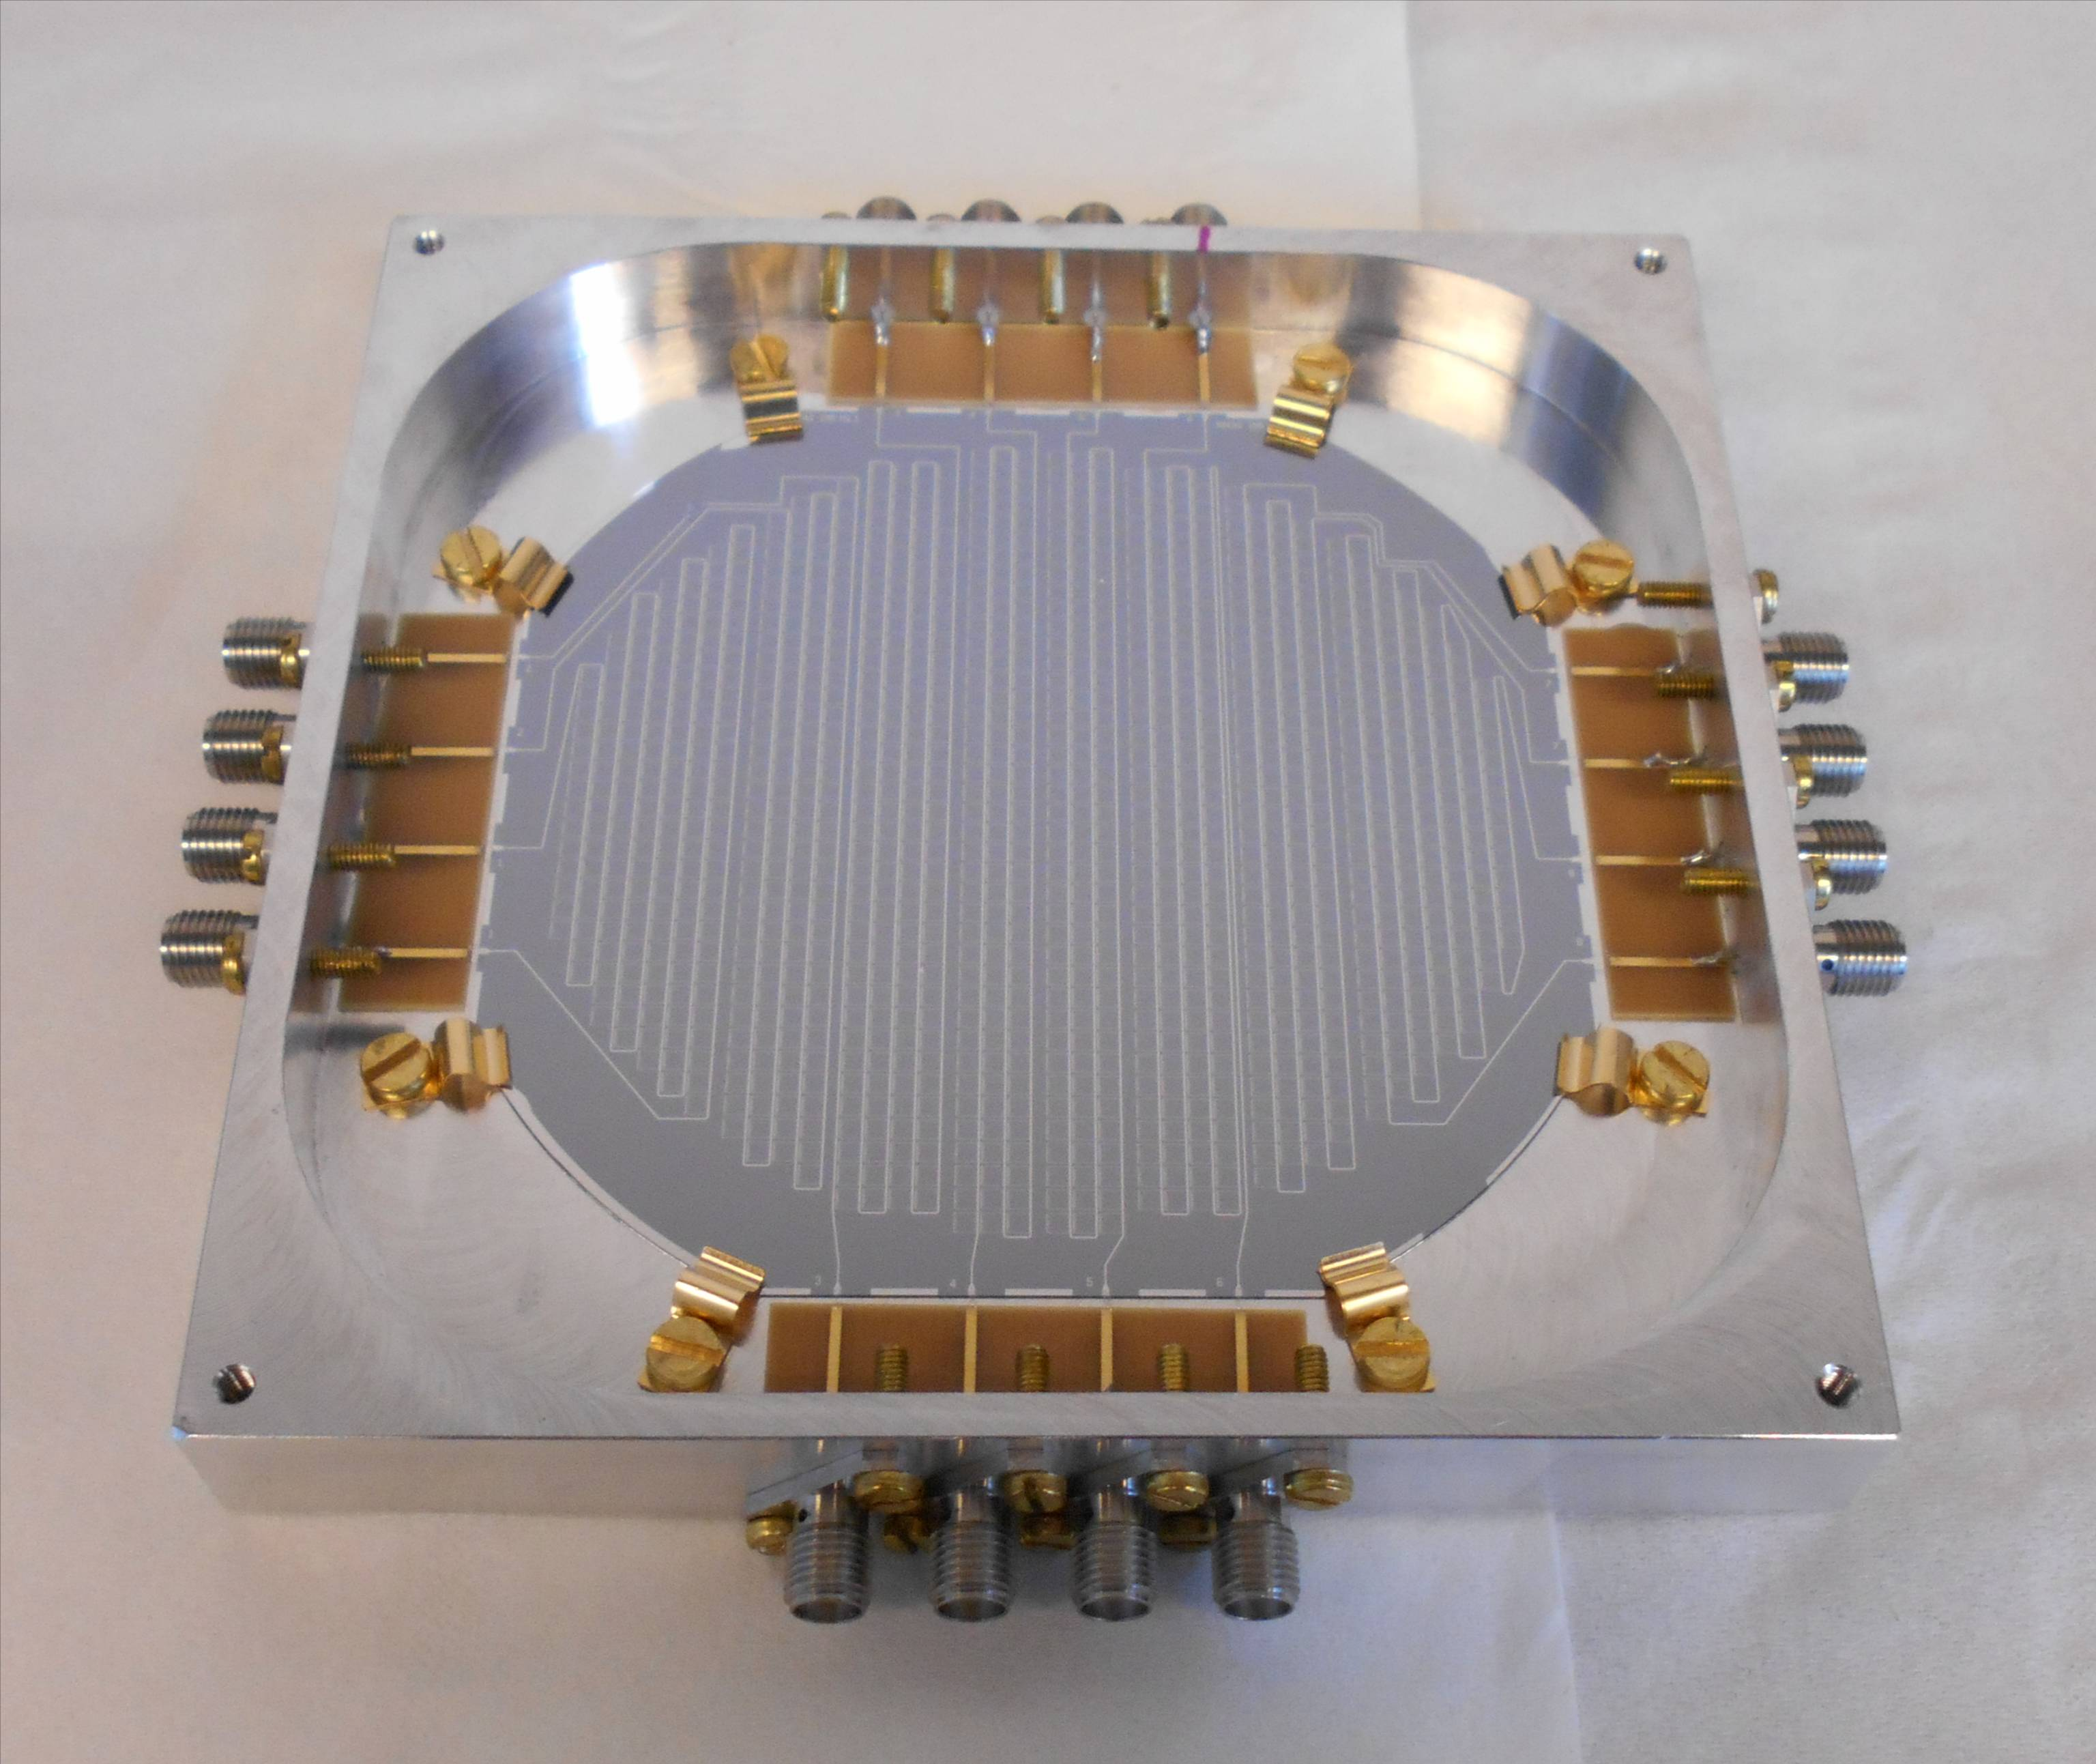
\includegraphics[clip, width=0.75\linewidth]{Figures/NIKA2/1mm_array.jpg}    
  \end{minipage}
  \hfill
  \begin{minipage}[c]{0.50\linewidth}
    \centering
     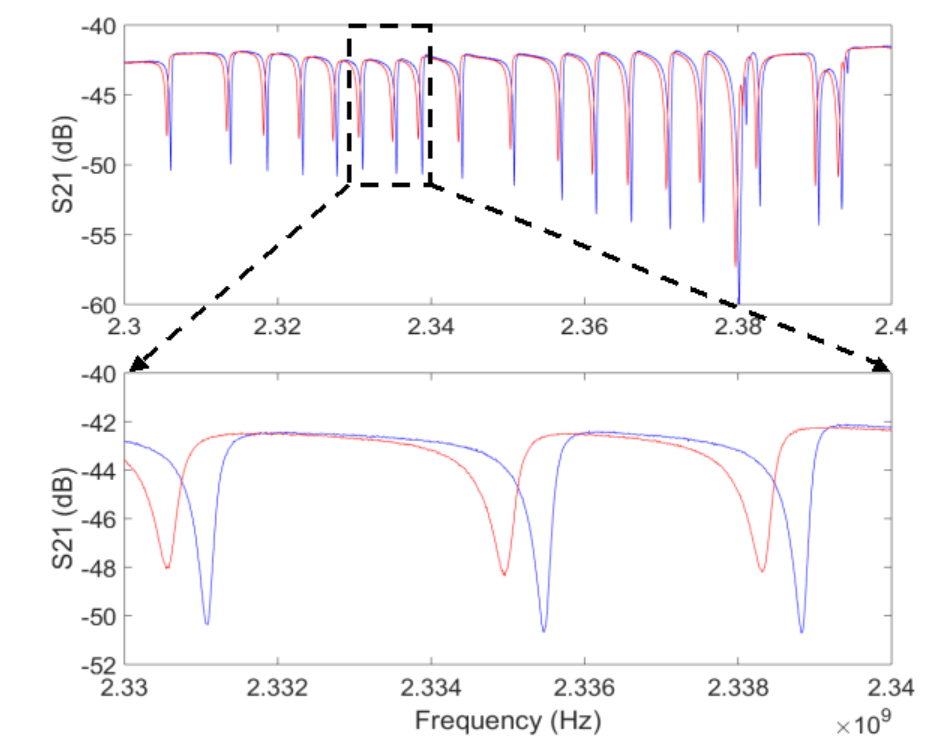
\includegraphics[clip, width=\linewidth]{Figures/NIKA2/260GHz-H_sky.png}
  \end{minipage}
  \caption{Les lignes de base et les données brutes. A gauche, une
    photo d'une des matrices à 1\,mm dans son support. On distingue
    les (8) lignes de base qui connectent chacun des (1140) KID, ainsi
    que les connecteurs d'entrée et de sortie de l'électronique
    froide. A droite est présenté un exemple de mesures des fréquence
    de résonance des KID effectuées en laboratoire. La figure du haut
    montre la fonction de transfert (paramètre de transmission $S_{21}$)
    mesurée à la sortie de l'une des lignes de base dans la bande à
    1\,mm, en effectuant un balayage en fréquence. La figure du bas
    présente un zoom isolant trois courbes de résonance typique. Sur
    les deux figures, les courbes bleues correspondent à la
    transmission des KID illuminés par un fond refroidi à 80\,K,
    tandis que les courbes rouges correspondent à une illumination à
    température ambiante (300\,K). Pour chacun des KID, la forme de la
    transmission varie et le minimum de transmission se décale en
    fréquence en fonction de la lumière reçue. Ces mesures sont
    utilisées pour estimer une réponse moyenne des KID à la
    température du ``ciel''dans~\citet{Adam2018}.}
  \label{fig:ma_fig}  
\end{figure}
 
Chaque bloc d'environ 150 KID est connecté à une même ligne de base
(cable co-axe) assurant la transmission du signal d'excitation en
entrée des détecteurs et la lecture du signal transmis en sortie des
détecteurs. La ligne d'excitation (entrée) et la ligne de lecture
(sortie) sont connectées directement sur la plaque de silicone à 150~mK
supportant les KID, au moyen de connecteurs dédiés (subminiature
version A, SMA). Le signal de sortie est dirigé vers un amplificateur
cryogénique à bas bruit (Low-noise amplificateur, LNA) spécialement
conçu pour NIKA2 (Observatoire \emph{Yebes} et entreprise \emph{TTI
  Norte} en Espagne). La matrice A2 est connectée à quatre lignes de
base tandis que huit lignes de bases équipent chacune des matrices à
1~mm, A1 et A3. Les connecteurs (SMA) d'entrée et de sortie pour l'une
des matrices à 1~mm sont visibles à la
figure~\ref{fig:ma_fig}. Cet ensemble, comprenant les connecteurs SMA,
le cables d'excitation et de lecture et les amplificateurs LNA forme
l'électronique froide, placée à l'intérieur du cryostat et faisant le
lien entre l'étage à 150~mK et la cabine du télescope (300~K).

Ensuite la production du signal d'excitation, la lecture des signaux
de sortie et les convertions entre signaux analogiques et digitales
pour les 2 900 détecteurs sont réalisés par une électrique de lecture
dédiée, développée pour NIKA et NIKA2 au LPSC à Grenoble. Cette
électronique, appelée \emph{New Iram Kid Electronic in Advanced
  Mezzanine Aard format} (NIKEL-AMC), se compose de 20 cartes
électroniques, chacune couvrant une bande de fréquence de 500~MHz et traitant
les signaux d'entrée et de sortie de 150 KID. Dans chaque bande de
500~MHz, le signal d'excitation est produit au moyen de cinq
convertisseurs digital-vers-analogique (DAC) couvrant chacun 100~MHz,
créant ainsi une sous-bande commune à une trentaine de KID.   
Les différentes cartes électroniques sont synchronisées entre elles et
avec le télescope de 30-m par un signal à un pulse par seconde (PPS)
fourni par le GPS du système de contrôle du télescope. Une description
détaillée de l'électronique de lecture de NIKA2 est donnée dans
\citet{Bourrion2012, Bourrion2016}.



\subsection{L'acquisition des données brutes}
\label{se:rawdata}

La photométrie avec des KID repose sur la mesure des variations de
leur fréquences de résonance, qui varient proportionellement à la
puissance optique reçue (voir Sect.~\ref{se:kid}). Les performances
des KID, utilisés comme détecteurs dans le domaine millimétrique, ont
été décrites théoriquement dans \citet{Swenson2010} et testées en
laboratoire avec les détecteurs de NIKA~\citep{Monfardini2014JLTP}. 

La mesure de la fréquence de résonance des KID se fait via la mesure
de la fonction de transfert entre le signal d'excitation envoyé en
entrée de la ligne de base et le signal transmis par les KIDs en
sortie. Un exemple de mesure de la fonction de transfert d'une série
de KID connectés à une même ligne de base, en fonction de la fréquence
du signal d'excitation est montré à la figure~\ref{fig:ma_fig}. La
résonance de chaque KID est repérées par un pic d'absorption du signal
d'entrée. Ainsi, chaque KID est associé à une fréquence
$f_{\rm{tone}}$, correspondant à sa fréquence de résonance pour une
puissance optique incidente de référence (définie, par exemple, en
occultant la fenêtre d'entrée du cryostat).

Les variations de fréquence de résonance des KID dues à la lumière
incidente $\Delta f$ se traduisent par des variations de leur fonction
de transfert complexe. Celle-ci est caractérisée par deux
quantités : une composante variant en phase avec le signal d'entrée,
notée $I$ (\emph{In-phase}) et une composante variant en quadrature,
notée $Q$ (\emph{in-Quadrature}). Il s'agit alors de relier les
quantités mesurées via le système d'acquisition de données, qui sont
les composantes de la fonction de transfert $I$ et $Q$ et ses
variations $\Delta I$ et $\Delta Q$, aux variations de fréquence de
résonance $\Delta f$. Pour cela, une méthode originale a
été développée pour NIKA et NIKA2, et est décrite dans
\citet{Calvo2013}.
Le signal d'excitation d'entrée est modulé à une fréquence fixée $df$,
où $df$ est très petit devant la largeur de la résonance. La mesure de
la variation de la fonction de transfert induite par ce décalage en
fréquence connu, $dI$ et $dQ$, nous permet de calibrer la relation
entre $\Delta I$ et $\Delta Q$ et $\Delta f$. Il est alors possible de
définir une quantité directement proportionelle à $\Delta f$. Cette quantité,
appelée \emph{RF\_dIdQ}, est définie comme la projection dans le plan
($I$, $Q$) du vecteur ($\Delta I$, $\Delta Q$) sur le vecteur ($dI$,
$dQ$). Cette quantité, proportionnelle à $\Delta f$ pour chaque KID,
constitue le signal ordonné en temps (\emph{Time Ordered Information},
TOI) des détecteurs. 
Ainsi, à partir des données brutes fournies par le système
d'acquisition, comprenant les quantités $I$, $Q$, $\Delta I$ et
$\Delta Q$, échantillonnées à $f_{\rm{sam}} = 23,4~\rm{Hz}$, pour
chaque KID, les TOI des KIDs sont construites. \'Etant
proportionnelles aux variations de fréquence de résonance, elles
s'expriment en Hz.

% ajouter un paragraphe sur le tuning ??
Finalement, pour maximiser la sensibilité des KID, le signal d'excitation
$f_{\rm{tone}}$ doit être proche de la fréquence de résonance. Or
celle-ci dépend du signal astrophysique mais aussi du bruit, dominé
par l'émission thermique de l'atmosphère. Le signal d'excitation doit
donc être adapté en temps réel, aux variations du rayonnement de fond 
d'origine atmosphérique, qui dépendent des fluctuations d'opacité de
l'atmosphère et de l'épaisseur d'atmosphère traversée sur la ligne de
visée, elle-même déterminée par l'élévation auxquelle se font les
observations. Pour cela, une procédure d'ajustement des
$f_{\rm{tone}}$, appelée {\tt tuning}, a été inclue à l'acquisition
de données~\citep{Adam2018}. Un {\tt tuning} est automatiquement
réalisé lorsque le télescope pointe vers une nouvelle source et au
début de chaque observation. Cette optimisation, qui ne prend que deux
secondes, permet de conserver une bonne sensibilité même dans des
conditions d'observation défavorables (forte opacité, instabilité de
l'atmosphère, observations à fort gradient d'élévation).



\subsection{Caractérisation en laboratoire}
\label{se:bandpass}

Une intense phase de caractérisation en laboratoire à l'Institut Néel
a précédée l'installation au télescope de 30-m de NIKA2, comme du
prédécesseur NIKA. Cette phase, qui a aussi mobilisée les équipes de
l'IPAG, l'IRAM et du LPSC a été cruciale pour l'élaboration du
dispositif instrumental final. En outre, deux bancs test originaux ont
été développés : un simulateur de ciel et un interféromètre
pour les mesures de bandes passantes.

Le simulateur de ciel, consistant en une bille mobile placée devant un
fond froid illuminant le plan focal via une lentille, est détaillé dans
\citet{Catalano2014, Monfardini2011_NIKA}. L'analyse des données issues de
"l'observation'' du simulateur de ciel a permis de tester les
performances des KID, d'optimiser les sous-systèmes instrumentaux, de
mettre en place et de tester le système d'acquisition et les outils de
traitement de données. Cette série de tests et les principaux
résultats obtenus pour NIKA2 sont résumés dans \citet{Adam2018}.


La caractérisation des bandes passantes de NIKA2 s'est effectuée au
moyen d'un interféromètre de Martin-Puplett (IMP) conçu à l'Institut
Néel~\citep{Durand2007_these}. L'IMP, couplé à une source de référence de
spectre de Rayleigh-Jeans, fournit un signal optique finement
sélectionné en fréquence. Ce signal dirigé à l'entrée du cryostat
vient illuminer le plan focal après avoir traversé le système optique
froid, permettant une mesure de la réponse spectrale en
transmission. Les bandes passantes pour chacunes des trois matrices de
détecteurs sont présentées à la
figure~\ref{fig:bandpass}. L'incertitude sur ces mesures permises
par le IMP est estimée meilleure que $1\%$. Les bandes
passantes de NIKA2 sont comparées à la transmission de l'atmosphère
pour deux contenus en vapeur d'eau (définis par la hauteur d'eau
précipitable ou \emph{precipitable water vapour}, pwv). Comme discuté
au paragraphe~\ref{se:optics}, la bande passante de A2 rempli bien la
fenêtre de transmission de l'atmosphère, tandis que les bandes
passantes de A1 et A3 tendent vers zéro vers 300~GHz pour limiter le
bruit atmosphérique dans les conditions d'observation moyenne à
médiocre.

\begin{figure}[ht!] 
\begin{center}
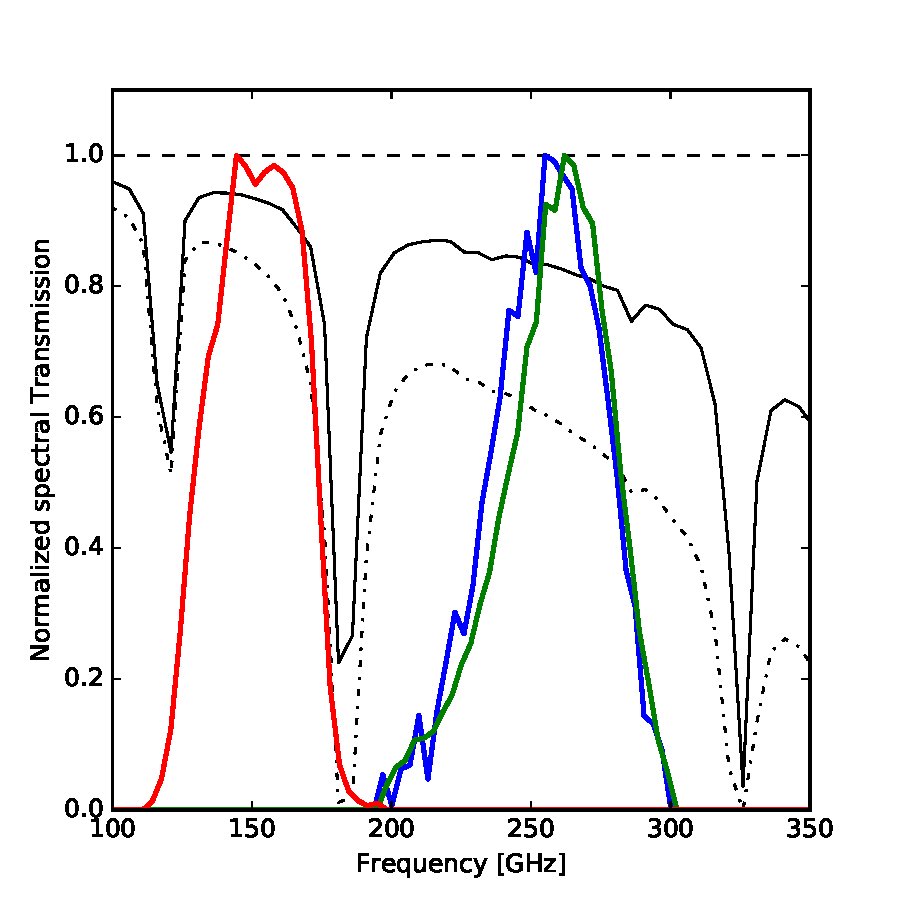
\includegraphics[clip,width=0.5\textwidth]{Figures/NIKA2/atm_transmission.pdf}
\caption[Les bandes passantes]{Les bandes passantes de NIKA2. La
  transmission spectrale de la matrice à 150\,GHz (A2 en rouge) et des
  deux matrices à 260\,GHz (A1, en bleu, et A3, en vert) est tracée en
  fonction de la fréquence. Ces courbes ont été mesurées au
  laboratoire dans un cryostat équipé de l'optique froide de NIKA2,
  incluant la première lame dichroïque installée (qui a été remplacée
  en 2016). Pour comparaison, la transmission de l'atmosphère,
  calculée à partir du modèle ATM\citep{Pardo2002}~, est également
  montrée pour deux valeurs de la hauteur d'eau précipitable (pwv) contenue
  dans l'atmosphère. La courbe en trait plein correspond à 2\,mm de
  pwv (bonnes conditions atmosphériques de semestres d'hiver), tandis que la courbe
  en trait discontinu correspond à 6\,mm de pwv (conditions moyennes
  d'observation de semestres d'été).} 
 \label{fig:bandpass}
\end{center}
\end{figure}

%%%%%%%%%%%%%%%%%%%%%%%%%%%%%%%%%%%%%%%%%%%%%%%%%%%%%%%%%%%%%%%%%%%%%%%
%
%
%
%
%             SECTION : OBSERVATIONS
%
%
%
%%%%%%%%%%%%%%%%%%%%%%%%%%%%%%%%%%%%%%%%%%%%%%%%%%%%%%%%%%%%%%%%%%%%%%%
\section{Observations au télescope}
\label{se:observations}

%\subsection{Le télescope de 30-m de l'IRAM}
Le télescope de 30-m de l'IRAM~\footnote{Science User's web pages: {\tt
  http://iram-institute.org/EN/content-page-55-7-55-0-0-0.html}}, en
opération depuis 1985, se situe à Pico Veleta
à 2870 mètres d'altitude, dans la Sierra Nevada espagnole. Ce site a
été choisi pour sa latitude suffisament basse (37 degré nord) pour
observer des sources jusqu'à une déclinaison d'environ -30
degrés sur le ciel et ses conditions météorologiques (sécheresse et
altitude). Le télescope est de type Nasmyth-Cassegrain, constitué d'un
miroir primaire parabolique équipé d'une monture
altazimutale~\citep{Baars1987}. Les instruments sont placés dans la
cabine \emph{Nasmyth}, située sous le miroir primaire et liée à
celui-ci en azimuth. La structure qui soutient le miroir primaire est conçue
suivant le principe homologique : elle minimise l'impact des
déformations du miroir sous l'effet de sont propre poids en le
contraignant a garder une forme parabolique à toutes les
élévations. De plus, l'ensemble du miroir primaire est thermalisé afin
de limiter les déformations dues aux variations de la température
extérieure~\citep{Baars1988}. Cette conception permet au télescope de
30-m d'offrir une résolution angulaire jusqu'à 10 arcsecondes et une
précision de pointage meilleure que 3 arcsecondes~\citep{Greve1996}.  


Le télescope de 30-m de l'IRAM est un observatoire ouvert à la
communauté scientifique. Des campagnes d'observations regroupant un
ensemble de projets scientifiques sélectionnés (\emph{observation
  pool}) sont organisées durant les semestres ``d'été''
(septembre à décembre) et "d'hiver'' (janvier à juin). Pour les
observations avec NIKA2, plusieurs de ces campagnes (de trois à cinq),
d'une durée d'une semaine, sont planifiées chaque semestre. Les
observations s'effectuent à partir de la salle de contrôle du 30-m en
passant une série d'instructions au système de contrôle du télescope
(\emph{New System Control}, NSC) concernant le pointage, le focus, et
la stratégie de balayage (\emph{scan}).
Pour la plupart des observations avec NIKA2, celle-ci
consiste à balayer continument le ciel dans les deux directions
suivant une coordonnées (azimuth, élévation, ascension droite,
déclinaison), tandis que la coordonnée perpendiculaire (élévation, azimuth,
déclinaison, ascension droite) est incrémentée d'un petit pas à chaque
changement de direction. Cette stratégie de balayage est appelée
\emph{On-the-Fly} (OTF) \emph{scan}. Un balayage continu dans une
direction est un \emph{subscan}. L'ensemble du scan couvre une zone de
ciel formant un rectangule (ou un parallèlogramme, un angle pouvant
être défini pour décaler le début de chaque subscan) dans le système
de coordonnées choisi. Plusieurs types de scans ont été optimisés pour les
observations de NIKA2 et sont utilisés lors des
campagnes techniques (commissioning) et scientifiques. Ils sont
décrits dans les sous-sections suivantes.

\subsection{Focus}
\label{se:focus}

Une session d'observation commence par l'optimisation du focus axial
du télescope, consistant à ajuster la position du miroir secondaire
selon l'axe optique, notée $z$. Pour cela, une procédure d'observation
dédiée a été développée pour NIKA2. Cette procédure consiste à
réaliser une série de cartes d'une source ponctuelle pour cinq
positions $z$ du miroir secondaire. Chacune des cartes est obtenue en
réalisant un petit scan OTF d'une durée d'une minute et couvrant une
zone de $1' \times 5'$ sur le ciel. Sur chacune des cartes, sont estimés
le flux de la source et la taille du lobe au moyenne d'ajustement de
Gaussiennes 2D. Les points de mesure du flux et de la résolution
angulaire sont ajustés par une parabole. Le meilleur focus est défini
comme la valeur qui maximise le flux et la résolution angulaire
mesurés pour les trois matrices de détecteurs.

Cette valeur de focus détermine le meilleur focus au centre du champ
de vue. En effet, étant donné la taille des cartes réalisées, ce sont
les détecteurs situés proches du centre des matrices qui contribuent le
plus à la mesure. Or, le champ de vue est suffisament étendu (6,5' de
diamètre) pour que la surface de meilleur focus ne soit pas plane mais
légèrement incurvée, de sorte que le meilleur focus au centre du champ
de vue soit sensiblement différent du meilleur focus à la
périphérie. Par conséquence, le focus du télescope peut être optimisé
de sorte de maximiser le nombre de détecteurs proches du meilleur
focus. Pour cela, nous avons mesuré les surfaces focales pour chacunes
des matrices de détecteurs, comme discuté dans~\citet{Perotto2019}. La
focalisation optimale des matrices est obtenue en décalant le meilleur
focus central de $-0.2~\rm{mm}$.

Comme les variations de température extérieure et d'illumation du
miroir primaire peuvent affectées le focus, une mesure de focus est
systématiquement réalisée aux levés et couchés du soleil, et ré-itérée
régulièrement durant la journée. 

\subsection{Pointage}
\label{se:pointing}

Le pointage consiste diriger exactement l'axe optique du
télescope vers un point dans le ciel. Le pointage du télescope de 30-m
repose sur un modèle de pointage dont les paramètres sont ajustés
plusieurs fois par an~\citep{Greve1996}. 

Une fois le télescope réglé au focus optimal (Sect.~\ref{se:focus}),
une procédure de correction de pointage est exécutée afin de faire
coïncider exactement le point de réference sur l'axe optique du
télescope avec le détecteur de référence de NIKA2. La plupart des
sources de pointage étant des sources radio (e.g. quasars), le
détecteur de référence est choisi au centre de la matrice A2
(150~GHz). Les corrections de pointage pour NIKA2 sont réalisées à
partir de scans dédiés vers une
source ponctuelle brillante. Un scan de pointage ({\tt pointing})
consiste à balayer la source en effectuant un aller-retour à azimuth
constant, puis à effectuer un second aller-retour à élévation
constante, formant ainsi une croix centrée sur la source et composée
de quatre subscans. La position de la source est mesurée à partir de
chacun des subscans. Les différences entre les deux positions mesurées
suivant chaque coordonnée sont utilisées pour dériver une
correction de pointage en azimuth et en élévation. 
 
\subsection{Skydip}
\label{se:skydip}

Un \emph{skydip} consiste à balayer un grand intervalle d'élévation à
azimuth constant dans le but de mesurer l'opacité de l'atmosphère en
faisant varier la masse d'air traversée sur la ligne de visée. 

Pour NIKA2, la variation de puissance optique reçue par les KID, dues
aux variations de la masse d'air avec l'élévation, est telle le décalage des
fréquences de résonance devient trop important pour le système
d'acquisition de données (voir Sect.~\ref{se:rawdata}). Par
conséquence, les \emph{skydip} de NIKA2 doivent s'effectuer pas-à-pas
par paliers en élévation successifs, au début desquels est réalisé un
{\tt tuning} des KID. Par ailleurs, les \emph{skydip} de NIKA2 ne sont
pas directement utilisés pour mesurer l'opacité instantanée de
l'atmosphère mais pour calibrer la réponse des KID aux variations de
transmission atmosphérique (voir Sect.~\ref{se:opacity}). Un {\tt skydip}
consiste en une série de 11 paliers en élévation placés entre 19 et 65
dégrés et régulièrement espacés en masse d'air. Le temps d'intégration
par paliers est de 20 secondes, pour une durée totale du {\tt skydip}
d'environ huit minutes.

\subsection{Beammap}
\label{se:beammap}

Les {\tt beammaps} vers des sources compactes très brillantes sont des
observations critiques pour la calibration de NIKA2. Il s'agit de
longs scans de type OTF définis pour permettre une mesure du lobe de
chaque détecteurs individuellement. Cette contrainte détermine les
paramètres du scan. Le scan est effectué en coordonnées équatoriales
($\az$, $\elev$) à élévation constante afin de minimiser les
variations de la transmission atmosphérique avec la masse d'air. En
coordonnées équatoriales ($\az$, $\elev$), le scan couvre un rectangle
de $13' \times 7.8'$, afin d'assurer que tous
les détecteurs observent complètement la source, même ceux situés
sur les bords des matrices. Un scan plus long dans la direction de
balayage permet une meilleure soustraction de bruit, en assurant un
nombre suffisant de détecteurs pointant loin de la source à chaque
instant. Pour échantillonner le lobe des matrices à 1~mm,
les subscans ne sont séparés que de 4.6'' et la vitesse de balayage
est fixée à 65 secondes par arcseconde, permettant des mesures
espacées de 2.7'' dans la direction de balayage, soit un
échantillonage meilleur que le critère de Nyquist. La durée de chaque
subscan est fixée à $12~\rm{s}$, proche de la durée minimale de
$10~\rm{s}$ imposée par le télescope de 30-m. En deça de cette limite,
le rapport du temps passé par le télescope à changer de direction par
rapport au temps d'observation utile devient prohibitif. L'observation
d'une {\tt beammap} dure environ 25 minutes. 



%%%%%%%%%%%%%%%%%%%%%%%%%%%%%%%%%%%%%%%%%%%%%%%%%%%%%%%%%%%%%%%%%%%%%%%
%
%
%
%
%             SECTION : COMMISSIONING
%
%
%
%%%%%%%%%%%%%%%%%%%%%%%%%%%%%%%%%%%%%%%%%%%%%%%%%%%%%%%%%%%%%%%%%%%%%%%
\section{Commissioning de NIKA2}
\label{se:commissioning}

\subsection{Historique du projet NIKA2 : le précurseur NIKA}
\label{se:nika}

L'aventure de NIKA2 débute avec le développement de l'instrument
précurseur, NIKA, à la fin des années 2000. En octobre 2009, la
première version de NIKA, alors équipé de 69 KID, voit sa première
lumière au télescope de 30-m de l'IRAM~\citep{Monfardini2010_NIKA}. Un
an plus tard, en octobre 2010, une campagne technique est organisée
pour tester NIKA dans une version proche de sa version finale. Il est
alors équipé 356 KID distribués dans deux matrices opérant à 150 et
260~GHz~\citep{Monfardini2011_NIKA}. Je rejoins le projet à l'automne
2011, d'abord pour effectuer les tests en laboratoire, puis pour
participer aux campagnes techniques au télescope de 30-m et à
l'analyse de données. Entre 2011
et 2014, sept campagnes techniques seront organisées. Les excellentes
performances de cet instrument prototype, décrites
dans~\citet{Catalano2014}, justifie l'organisation de trois campagnes
scientifiques au 30-m de l'IRAM sur sélection de projets d'observation
en 2014 et 2015. La calibration et
la livraison des données aux observateurs est alors à la charge de la
collaboration NIKA et est réalisée par les équipes de l'IPAG et du
LPSC. En parallèle, l'instrument NIKA2 est construit et testé sous
la coordination de l'Institut Néel. En janvier 2015, j'intègre
l'équipe c\oe eur (\emph{Core Team}) de la collaboration NIKA-NIKA2. Les
observations avec NIKA ont donné lieu à une série de publications
d'intérêt astrophysique et cosmologique dans les domaines des amas de
galaxies~\citep{Adam2014, Adam2015, Adam2016, Adam2017, Adam2017kSZ,
  Adam2018, Ruppin2017, Romero2018}, de l'émission diffuse
galactique et la formation stellaire~\citep{Bracco2017, Chacon2017,
  Rigby2018} et de la polarisation~\citep{Ritacco2018}.

\subsection{Déroulé du commissioning de NIKA2}
\label{se:historic}

\subsubsection{L'installation au 30-m}
A l'issu des tests en laboratoire, NIKA2 est installée au télescope de
30-m, comme décrit dans~\citet{Adam2018}, et voit sa première lumière,
avec une partie seulement de l'électronique de lecture, en octobre
2015. La première campagne d'observations techniques avec une lecture
des trois matrices au complet est réalisée en janvier 2016.

\subsubsection{Optimisation du dispositif instrumental}
La campagne suivante, appelé \emph{NIKA2 Run 4} (\emph{N2R4}), en mars
2016, est exempte d'incidents techniques et marquée par une météo
favorable. En particulier, les observations effectuées alors,
permettent une mesure précise des surfaces focales des trois matrices
(voir Sect.~\ref{se:focus}) et la mise au jour d'une courbure
inexpliquée de la surface focale de la matrice A2. N'impactant qu'une
des deux bandes de fréquence, cette courbure est attribuée à une
déformation (défaut de planéité) de la lame dichroïque. Une
intervention sur l'instrument est organisée en
septembre 2016, au cours de laquelle est installée une lame dichroïque
utilisant une nouvelle technologie robuste aux
déformations induites par les très basses températures
(Sect.~\ref{se:optics}). De plus, afin d'améliorer la sensibilité de
l'instrument, les lentilles placées immediatement devant les matrices
sont remplacées par de nouvelles lentilles corruguées pour limiter
les pertes de lumière par reflection, et la matrice A2 est remplacée
par une nouvelle matrice ayant démontrée une meilleure sensibilité
lors des tests en laboratoire. Par ailleurs, je deviens officiellement
responsable du commissioning et de la caractérisation des performances
en septembre 2016.

\subsubsection{Fin des modifications instrumentales}
Après l'intervention de septembre 2016, les surfaces focales mesurées
sont en accord avec les prédictions issues de simulations optiques pour
les trois matrices, validant ainsi l'absence de déformations de la
nouvelle lame dichroïque. En revanche, les mesures des gains des
détecteurs (\emph{flat field}) révèlent un gradient significatif dans
le champ de vue de l'une des matrices à 1 mm. Il s'agit de la matrice
A1, illuminée par la composante de polarisation transmise par le
polariseur (Sect.~\ref{se:matrices}). Trois origines sont possibles
pour cet effet : un défaut de transmission de l'une des composantes de
polarisation par la lame dichroïque, un défaut de réalisation de la
lentille corruguée placée devant la matrice A1, un désalignement du
faisceau illuminant A1 suite à l'intervention de septembre. En janvier
2017, une nouvelle intervention sur l'instrument est organisée, au
cours de laquelle les lentilles lisses sont re-installées et
l'alignement optique ré-ajusté finement. Les observations techniques
effectuées après l'intervention (durant \emph{N2R8}) révèlent 1) une
amélioration de la forme des lobes des détecteurs de la matrice A1 due
au meilleur alignement optique et 2) un gradient des gains des
détecteurs de A1 inchangé. Par élimination, cette intervention a
confirmé le défaut de transmission de la lame dichroïque. Au vue de
bonnes performances de NIKA2 par ailleurs (voir Chapitre II),
le dispositif instrumental a été figé.

\subsubsection{Phase finale du commissioning}
En février 2017 a lieu la première campagne technique avec
l'instrument final, le \emph{NIKA2 Run 9} (\emph{N2R9}). Avec pour
objectifs de finaliser la phase de commissioning, publier les
résultats du commissioning et caractériser l'instrument, j'ai
constitué une équipe dédiée, la \emph{Commissioning Tiger Team},
réunissant les principaux contributeurs à l'analyse des données parmi
les membres de la collaboration NIKA2. Une dernière campagne technique
a été organisée en avril 2017 (\emph{NIKA2 Run 10} ou \emph{N2R10}),
incluant une phase de vérification scientifique (SVP) de 30
heures. Après un appel à propositions d'observation
au sein de la collaboration, trois projets ont été retenus :
l'observation d'une galaxie proche (M99), d'un amas de galaxie du
\emph{Large Program} SZ (voir Chapitre III), et d'une source
présentant un possible disque de débris (GJ526). En dépit de
conditions météorologique défavorables et d'un sous-système de la
chaine cryogégique dégradé (turbo pompe en fin de vie), cette campagne
a été couronnée de succès, les observations de la SVP donnant lieu à
la première publication scientifique (non-technique) de
NIKA2~\citep{Ruppin2018}. Une première caractérisation de l'instrument,
s'appuyant sur l'analyse des données du N2R9 et N2R10, a été publiée
dans~\citet{Adam2018}.

\subsubsection{Calibration et caractérisation des performances}
La fin de la phase de commissioning a été officialisée en septembre
2017 à l'issue de la revue des performances par l'IRAM. NIKA2 est
alors devenu un instrument à demeure du télescope de 30-m, ouvert à la
communauté scientifique, sous responsabilité de
l'IRAM. Toutefois, une condition a été ajoutée par l'IRAM pour acter
la livraison de l'instrument, stipulant que soit remis un document
détaillant la calibration et les performances de NIKA2.  

La première campagne scientifique de NIKA2, le \emph{NIKA2 Run 12}
(N2R12), a eu lieu en octobre 2017. L'analyse des données dédiées à la
calibration a mis au jour un manque de flux mesuré sur le calibrateur
secondaire le mieux connu (MWC349). En janvier 2018, ce fut la première
campagne d'observation scientifique d'hiver, aussi appelée \emph{NIKA2
Run 14} (N2R14), bénéficiant de conditions d'observation
stables. A partir des données du N2R14, une variation
journalière du lobe de l'instrument (voir Sect.~\ref{se:beam}) a été
mise en évidence. Cet effet, impactant aussi le flux mesuré, est
compatible avec le flux manquant des calibrateurs secondaires observés
au N2R12. Après correction de l'effet du lobe, une variation
résiduelle (15\%) du flux avec l'opacité de l'atmosphère est observée,
indiquant la présence d'un effet systématique. A l'issue d'une intense
phase de tests des effets systématiques, émerge une méthode de
calibration de référence, assurant une bonne stabilité des flux
mesurés : la calibration \emph{baseline}.

\subsubsection{Début de l'exploitation scientifique}
En juillet 2018, notre équipe livre un \emph{pipeline} de calibration
des données de NIKA2 à l'IRAM. Dorénavant, la calibration est prise en
charge par le responsable des observations avec NIKA2 au télescope de
30-m (Bilal Ladjelate). Nous détaillons la méthode de calibration et
compilons les performances de l'instrument dans le document
\emph{commissioning} (130 pages), remis à l'IRAM en décembre 2018. Ces
méthodes et résultats donnent lieu à un article de référence de
la collaboration NIKA2~\citep{Perotto2019}, soumis pour publication en
juillet 2019. Depuis octobre 2017, NIKA2 totalise 18 campagnes
d'observation scientifiques au télescope de 30-m. La première
conférence internationale\footnote{\emph{Millimeter Universe with NIKA2},
  \url{https://lpsc-indico.in2p3.fr/Indico/event/1765/}} dédiée à
l'exploitation scientifique des données de NIKA2 a réuni 75 personnes
en juin 2019 au LPSC. NIKA2 restera en opération au 30-m au
moins jusqu'en 2030.


\subsection{Organisation du travail}

J'ai pris la responsabilité du commissioning de NIKA2 en septembre
2016. Le défi majeur alors était de faire collaborer les équipes de
NIKA2 spécialistes de l'analyse de données avec des KID (IPAG et LPSC)
et les équipes de l'IRAM, à vocation à livrer les données calibrées de
NIKA2 aux observateurs externes, et d'interesser aux problématiques
d'analyse de données, les équipes ayant construit l'instrument
(e.g. Institut Néel). L'enjeu était critique du à la nécessité de
partager information et expertise entre NIKA2 et l'IRAM d'une part, et
les experts de l'analyse et de l'instrument d'autre part. J'ai donc
repris l'animation de la réunion hebdomadaire de NIKA2, à la suite de
Nicolas Ponthieu (à qui cette tâche délicate incombait depuis deux
ans), avec une approche pro-active pour inciter chaque partie a
participer et présenter des résultats. En outre, j'ai mis en place ou
ré-organisés des outils de travail collaboratifs, dont une série de
pages wiki. Ce wiki comprenait en particulier un espace
\emph{notebook} pour accueillir la description des analyses réalisées
par chacun. Plus de 90 études ont été postées sur cet espace, qui
s'est avéré un outil efficace pour échanger l'information et garder
une trace des résultats obtenus. Ce système de notes internes,
rassemblées dans les pages wiki et discutées en réunion de
collaboration a été crucial pour dépister les problèmes, puis définir
les tests à effectuer lors des campagnes d'observations techniques.

Une fois le dispositif expérimental figé (janvier 2017) et pour
finaliser la phase de commissioning, la difficulté a été de lutter
contre la dispersion des efforts et des pistes d'analyse explorées
pour concrétiser une caractérisation complète de l'instrument. Dans ce
but, j'ai rassemblé les principaux contributeurs de la collaboration
NIKA2 à l'effort d'analyse de données pour former une équipe dédiée à
la caractérisation de l'instrument, la \emph{Commissioning Tiger
  Team}. Celle-ci a réuni sept chercheurs du LPSC, IPAG,
Service d'Astrophysique du CEA et Observatoire de Paris et un
doctorant. Nous avons adopté des méthodes de travail, qui ont été
cruciales pour l'obtention des résultats finaux. Une réunion
hebdomadaires d'une durée maximale de deux heures a été mise en
place. Ensemble, nous avons d'abord identifié les principaux
\emph{challenges} et les points
bloquants, puis nous sommes partagé les tâches dont l'avancement a été
assuré par un suivi des "actions'' attribuées à chacuns. Notre travail
s'est structuré en découpant la calibration et la caractérisation des
performances par blocs (donnant sa structure au chapitre II). Pour
tester la stabilité des données sur plusieurs campagnes, nous avons
défini des méthodes de référence (et partagé les codes
correspondants). Inversement, des jeux de données de référence ont été
définis pour comparer les différentes méthodes développées. Enfin, en
collaboration avec l'IRAM, nous avons défini une liste de
critères de performance de l'instrument à caractériser, comprenant les
pré-requis définis dans le \emph{Memorandum of Understanding} (MoU),
mais aussi une liste de caractéristiques à tester, émergeant des
études ménées sur les données depuis 2016. 

Entre janvier 2017 et décembre 2018, l'essentiel du développement des
méthodes de calibration et d'estimation des performances s'est
effectué au sein de la \emph{Commissioning Tiger Team}. Nos travaux se
sont concrétisés dans plusieurs réalisations : une première
caractérisation des performances décrites dans~\citet{Adam2018}, puis
présentée à la revue des performances de l'IRAM, le développement et
la mise à disposition d'un \emph{pipeline} de calibration des données,
l'écriture du document \emph{Commissioning\&Performance} (130 pages)
accompagnant la livraison de l'instrument à l'IRAM, écriture d'un
article de référence compilant la description des méthodes et des
résultats du commissioning~\citep{Perotto2019}. 



\subsection{Définition d'un jeu de données de référence}
\label{se:scan_selection}

Le développement des méthodes de calibration et la caractérisation
des performances se sont effectuées conjointement au début de
l'exploitation scientifique, alors que quatre campagnes d'observations
étaient organisées par semestre. Afin de cristalliser ce processus, il
est apparu nécessaire au début 2018, de définir un jeu de données de
référence à partir duquel seront testées les méthodes et dérivés les
résultats finaux. Ce jeu de données devait être suffisament restreint
pour permettre des tests de robustesse extensifs, mais assez étendu
pour couvrir l'ensemble des conditions d'observation rencontrées sur
le site.

Le jeu de données de référence pour la caractérisation des
performances inclut les observations acquises lors de trois campagnes
: N2R9, la première campagne technique avec le dispositif
instrumental final; N2R12, la première campagne scientifique
organisée pendant un semestre d'été; N2R14, la première campagne
scientifique de semestre d'hiver. Ces trois campagnes couvrent un
intervalle de plus d'un an, garantissant la représentativité des
conditions d'observation au 30-m. Chacune des campagnes d'observation
représente un temps d'observation total d'environ 150 heures réparti
en 1300 scans d'observation environ d'une durée comprise entre
deux et 30 minutes.

Ensuite, pour refléter les performances de l'instrument pour une
exploitation scientifique, nous avons défini une sélection des scans
visant à exclure les conditions d'observations extrêmes. Nous avons
adoptés des critères simples et peu contraignants, portant sur l'opacité
atmosphérique au zenith mesurée dans les bandes de fréquence de NIKA2,
$\taunu$ et sur l'élévation des observations, $\elev$. Précisément,
les scans retenus doivent vérifier :
\begin{itemize}
  \item[i)]{$\tau_{A3} < 0.5$, où $\tau_{A_3}$ est $\taunu$ mesuré
    avec la matrice A3, correspondant à une atténuation atmosphérique
    du flux d'un facteur deux à une élévation de $45\degree$;}
  \item[ii)]{$\elev < 20\degree$, afin de limiter l'impact des deformations du lobe
    sous l'effet de la gravité;}
  \item[iii)]{$x\, \taunu < 0.7$, où $x = 1/\sin(\elev)$ représente la
    masse d'air traversée sur la ligne de visée, correspondant à une
    atténuation atmosphérique du flux d'un facteur deux.}
\end{itemize}

Ces critères n'excluent qu'une petite fraction des scans observés lors
des trois campagnes de référence. {\color{bleu}{ESTIMER CETTE
    FRACTION ?}}
Par ailleurs, pour des raisons d'instabilités liées à la température
extérieure, qui seront explicitées plus avant à la
Sect.~\ref{se:fwhm_variations}, nous excluons les observations
acquises entre 9\,h et 10\,h UTC, correspondant au lever du Soleil,
ainsi que celles de l'après-midi, entre 15\,h et 22\,h UTC. L'ensemble
de ces critères de sélection définit la sélection \emph{baseline}. 

